\documentclass[]{beamer}
% \usepackage{extsize}
\usepackage{minted}
\usepackage{pgfplots}
\usemintedstyle{fruity}
% \usepackage{subcaption}
\usepackage[size=a3,orientation=portrait,scale=1.8]{beamerposter}
\usepackage[citations,footnotes,definitionLists,hashEnumerators,smartEllipses,tightLists=false,pipeTables,tableCaptions,hybrid,outputDir={../..}]{markdown}
% \usepackage{expl3}
% \usepackage{ragged2e}

\usetheme{poster}
\graphicspath{{../images/}}

\definecolor{vsblue}{HTML}{007ACC}
\definecolor{vsactivebg}{HTML}{252526}
\definecolor{vsbg}{HTML}{1C1C1C}
\definecolor{vsgreen}{HTML}{62B455}
\definecolor{vsred}{HTML}{B1383B}
\definecolor{vsyellow}{HTML}{E5AD34}
\definecolor{vsgrey}{HTML}{3c3c3c}

\setbeamercolor{background canvas}{bg=vsbg,fg=white}
\setbeamercolor{alerted text}{fg=vsred}
\setbeamercolor{structure}{fg=vsgrey}
\setbeamercolor{palette primary}{fg=white,bg=vsblue}
\setbeamercolor{palette secondary}{fg=white, bg=vsactivebg}
\setbeamercolor{palette quarternary}{fg=white, bg=vsactivebg}
\setbeamercolor{headline}{fg=white,bg=vsgrey}
\setbeamercolor{title in headline}{fg=white}
\setbeamercolor{footline}{fg=white,bg=vsblue}
\setbeamercolor{foot}{bg=vsblue,fg=white}
\setbeamercolor{author in footline}{fg=white}
\setbeamercolor{institute in footline}{fg=white}
\setbeamercolor{separation line}{bg=white,fg=black}
\setbeamercolor{block body}{bg=vsactivebg,fg=white}
\setbeamercolor{block title}{fg=white,bg=vsblue}
\setbeamercolor{itemize item}{fg=vsyellow}
\setbeamercolor{itemize subitem}{fg=vsyellow}
\setbeamercolor{enumerate item}{fg=vsyellow}
\setbeamercolor{enumerate subitem}{fg=vsyellow}
% \renewcommand{\familydefault}{\sfdefault}

\usepackage[utf8]{inputenc}
\usepackage[T1]{fontenc}
% \usepackage{libertine}
% \usepackage[scaled=0.92]{inconsolata}
% \usepackage[libertine]{newtxmath}
\usepackage[numbers]{natbib}
\renewcommand{\bibfont}{\small}

\newcolumntype{b}{X}
\newcolumntype{s}{>{\hsize=.5\hsize}X}


%%begin novalidate
\ExplSyntaxOn
\markdownSetup{
    fencedCode,
    % html=true,
    rendererPrototypes={
        link = {\href{#2}{#1}},
        headingFour = {\begin{block}{#1}},
        horizontalRule = {\end{block}},
        % image = {
        %     \begin{figure}
        %         \centering
        %         hello
        %         \includegraphics{#3}
        %     \end{figure}
        % }
    },
    % renderers = {
    %     linkAttributeContextBegin = {
    %       \group_begin:
    %       \markdownSetup{
    %         renderers = {
    %           attributeKeyValue = {
    %              \setkeys
    %                { Gin }
    %                { {#1} = {#2} }
    %           },
    %         },
    %       }
    %     },
    %     image = {
    %       \includegraphics
    %         { #2 }
    %     },
    %     linkAttributeContextEnd = {
    %       \group_end:
    %     },
    % },
}
\ExplSyntaxOff
%%end novalidate

\author[under the supervision of Dr. Tim Storer]{Inesh Bose}
\title{Holistic Dashboard of Software\\Development Work-Time \& Practices}
\institute{University of Glasgow \hspace{1.8cm} \textit{\scriptsize Poster design inspired by \textbf{VSCode Dark theme}}}
% Optional foot image
\footimage{
\includegraphics[]{uog_white.pdf}}

\begin{document}

\begin{frame}[fragile]\centering

% \vspace{-5cm}

\begin{columns}
\begin{column}{0.57\textwidth}

\begin{markdown}

#### Introduction {\scriptsize what's this?}

Have you been developing software using \textcolor{yellow}{professional practices}* for a while? Have you worked in an \textcolor{lime}{agile team}? Have you experienced \textcolor{red!70}{project failure}? Do you tend to fight your \textcolor{cyan!80}{development environment} more than developing the project?

\vspace{0.4cm}

{\small There are good chances that you may be facing frustration due to poor Developer Experience. It is essential to realise that humans are the most important aspect of Software Engineering [@martinAgileSoftwareDevelopment2003]. Task estimation may be over-optimistic also affecting the project budget, and educating estimates requires knowledge of productivity by choosing the right metrics [@trendowiczChapterFactorsInfluencing2009].}

\vspace{0.4cm}

{\footnotesize {*} - such as branching, CI/CD, \& issue management with effort estimation using story points}

----
\end{markdown}
\end{column}

\begin{column}{.4\textwidth}
\begin{markdown}

#### Technologies \& APIs

- VSCode Webview API
- SvelteKit + Vite
- Chart.js + Typed Schemas
- GitHub API Plugin {\footnotesize (+ UofG SoCS GitLab)}
- WakaTime API Plugin

\vspace{0.5cm}

| \hspace{0.05cm} 
\includegraphics[width=0.14\textwidth]{vscode_logo.png} | \hspace{0.06cm} 
\includegraphics[width=0.12\textwidth]{svelte_logo.png} | 
\includegraphics[width=0.14\textwidth]{chartjs_logo.png} | 
\includegraphics[width=0.14\textwidth,decodearray={1 0 1 0 1 0}]{github_logo.png} | 
\includegraphics[width=0.14\textwidth,decodearray={1 0 1 0 1 0}]{wakatime_logo.png}
|---|---|---|---|---|
% | {\footnotesize VSCode} | {\footnotesize SvelteKit} | {\footnotesize Chart.js} | {\footnotesize GitHub} | {\footnotesize WakaTime} |

\vspace{0.8cm}

{\footnotesize Additional dev-dependencies include turbo, nitropack \& esbuild.} 

----
\end{markdown}
\end{column}

\end{columns}

\medskip
{\usebeamercolor[bg]{headline}\hrulefill}
\medskip

\begin{markdown}

#### Background \& Literature Survey {\scriptsize why's this?}

\small

Through this project, we aim to understand Developer Experience (DX) since it is believed that \textcolor{vsyellow}{eliminating frustrations in DX can promote productivity} \cite{mullerStuckFrustratedFlow2015} and help products \cite{sommervilleSoftwareEngineering1992} deliver good User Experience (UX). The increase in the industry, with more engineers and open-source software, is \textcolor{vsgreen}{causing Developer Relations \& DX to become an important aspect}, but another critical area is estimating tasks; with a varied workforce \& a limited budget, inaccurately measuring efforts can frustrate developers with the project.

\vspace{-0.5cm}

| \begin{figure}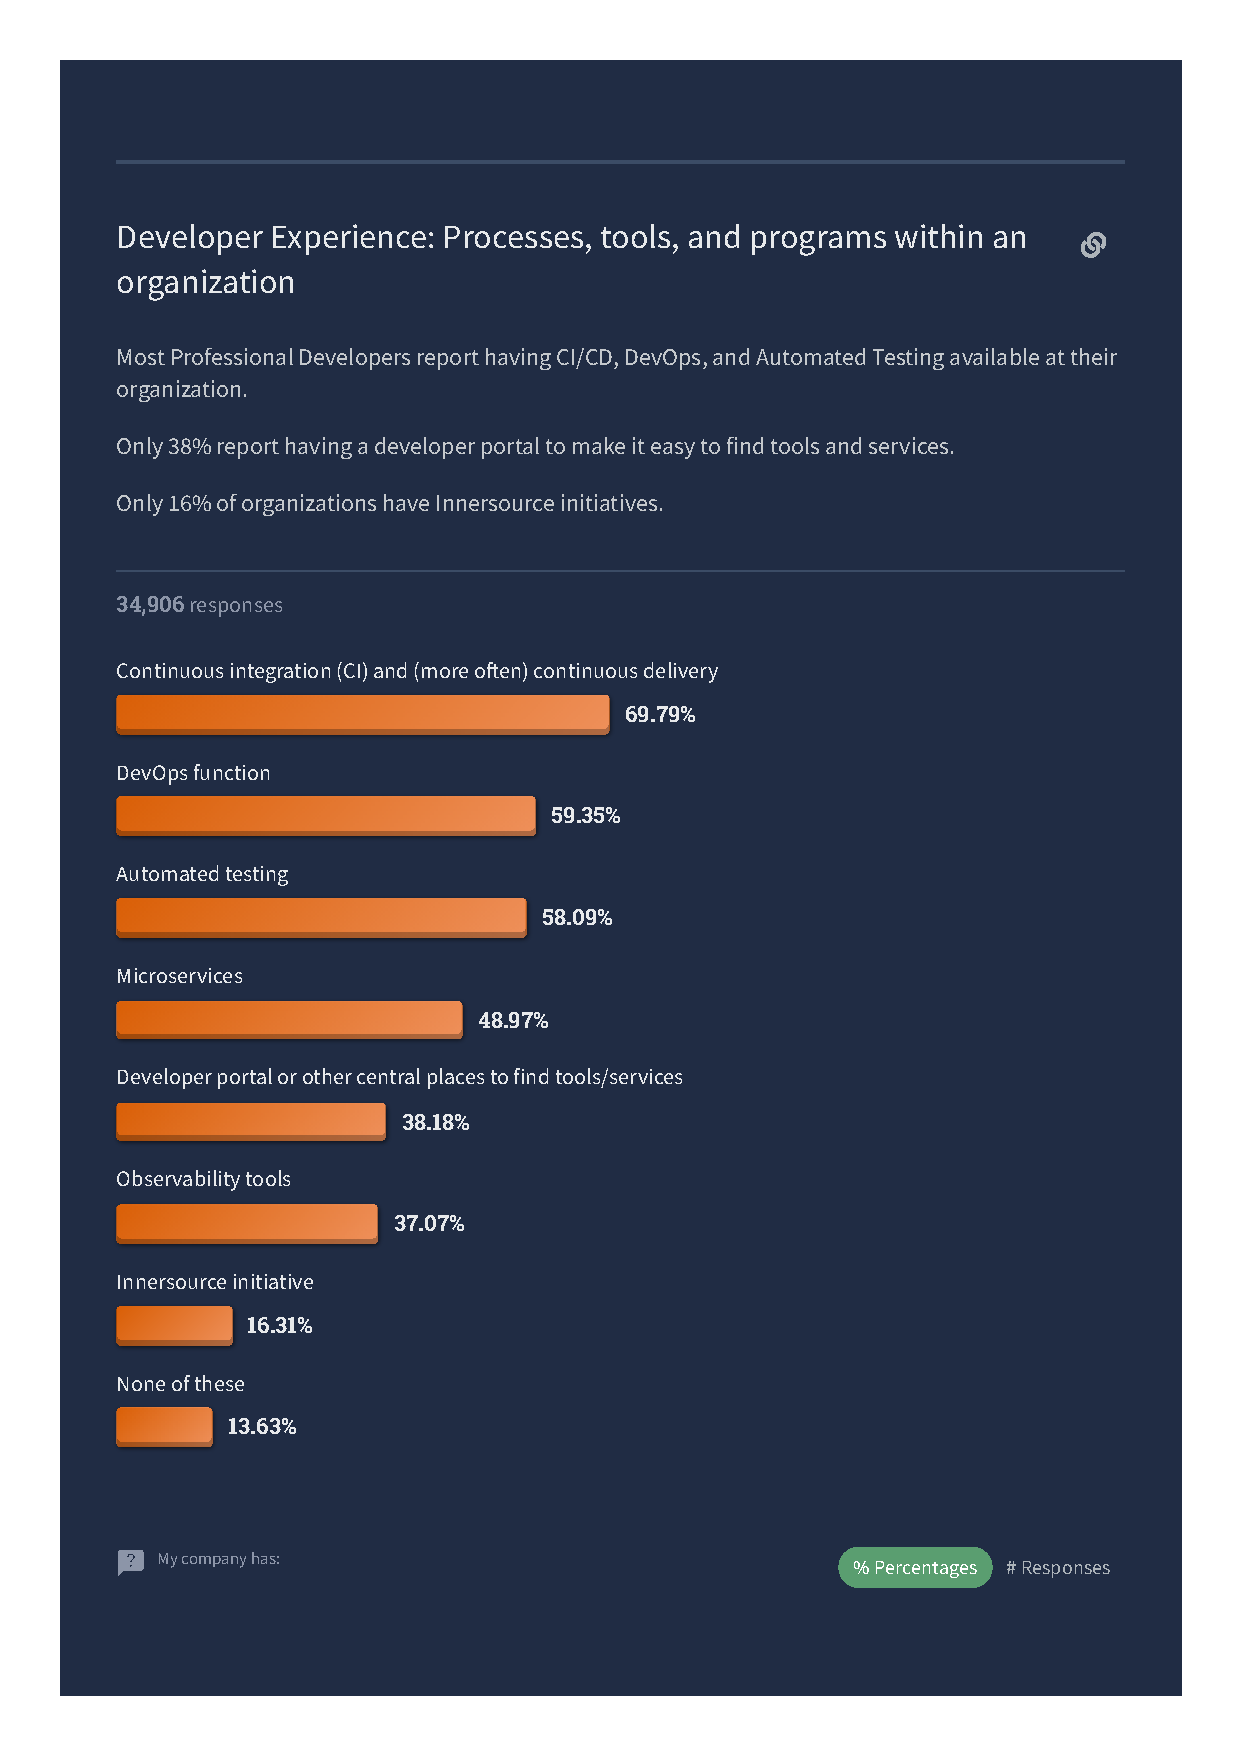
\includegraphics[width=0.38\textwidth,trim={0 20cm 0 2cm},clip]{Stack Overflow Developer Survey 2022.pdf}\end{figure} | \begin{figure}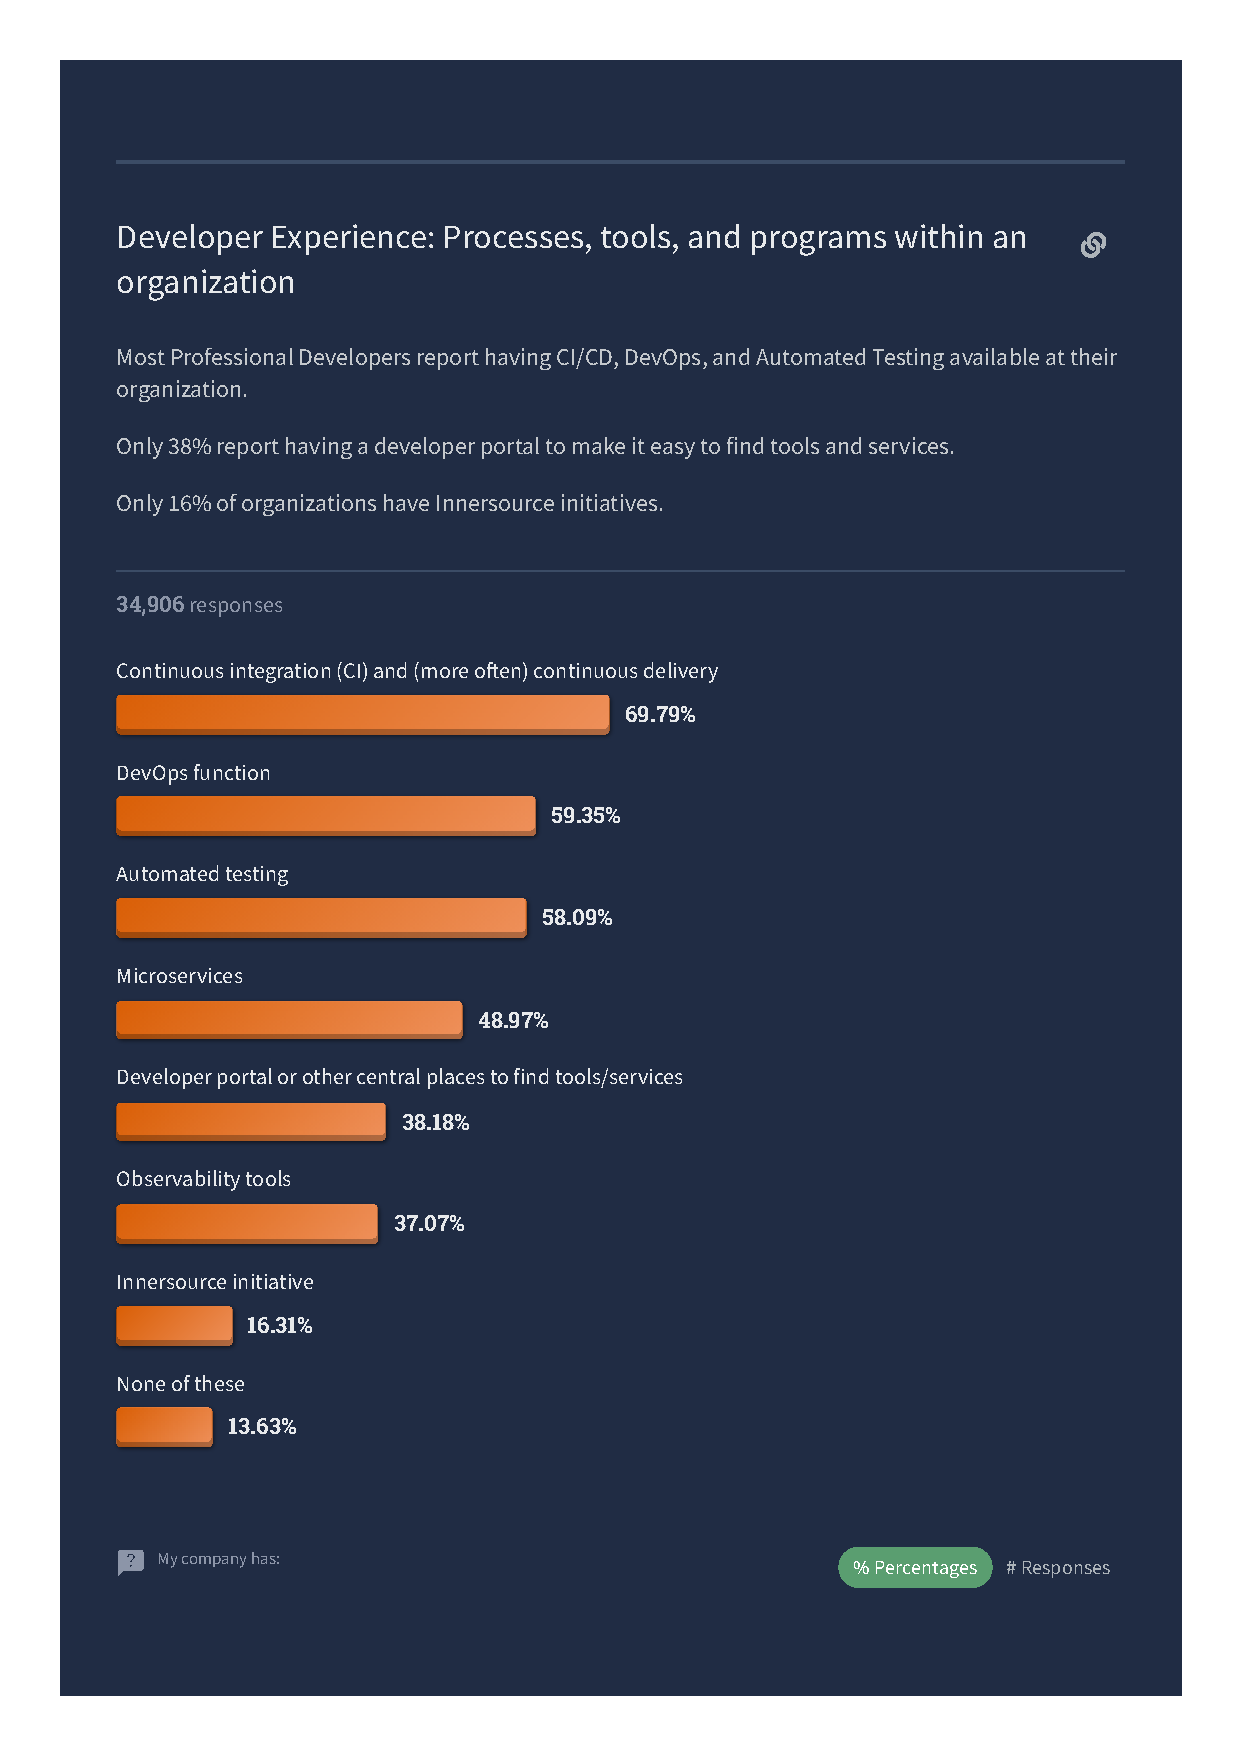
\includegraphics[width=0.38\textwidth,trim={0 13.5cm 0 9cm},clip]{Stack Overflow Developer Survey 2022.pdf}\end{figure} | \begin{figure}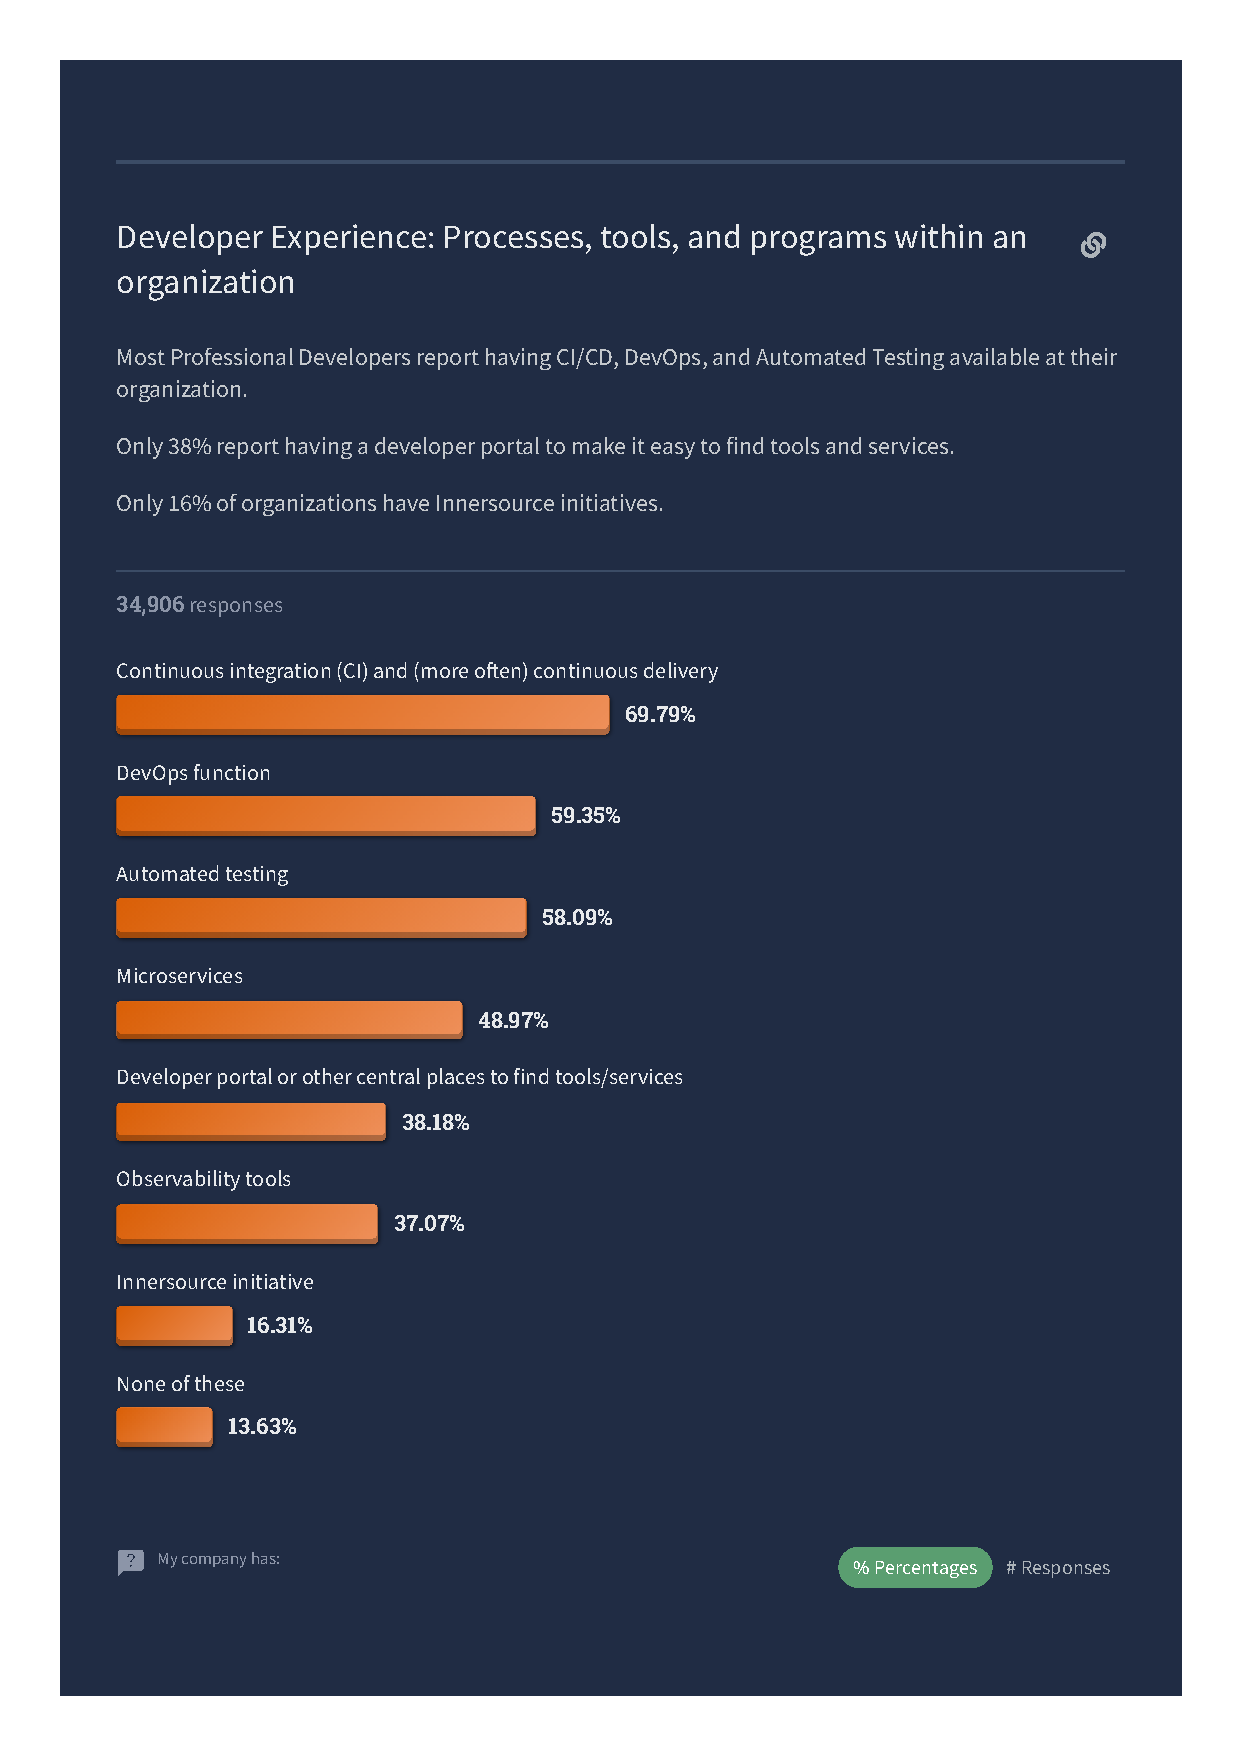
\includegraphics[width=0.38\textwidth,trim={0 6.5cm 0 16cm},clip]{Stack Overflow Developer Survey 2022.pdf}\end{figure} |
| --- | --- | --- |

\vspace{-0.5cm}

----

\end{markdown}

\vspace{-0.6cm}

\begin{columns}[T]

%%%% First Column
\begin{column}{.48\textwidth}

\begin{markdown}

#### Design \& Implementation {\scriptsize how's this?}

\footnotesize

Humans interact with computers using interfaces \cite{liCategorisationVisualisationMethods2016}; developers use an IDE that provides a \textcolor{red!30}{Text Editor} to provide a lower-level form of instructions to the computer. Using the technologies listed, we develop an \textcolor{yellow}{embedded modular} \textcolor{cyan}{dashboard into Visual Studio Code} that would be \textcolor{lime}{evaluated over 52 weeks}.

\vspace{-0.5cm}

| \begin{figure}\textcolor{black}{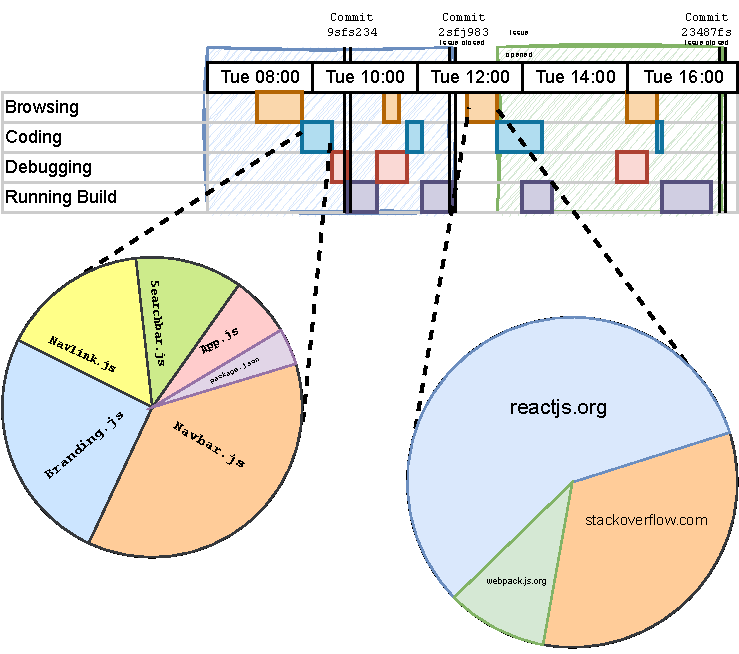
\includegraphics[width=0.38\textwidth]{sampleviz.pdf}}\end{figure} | \begin{figure}\textcolor{black}{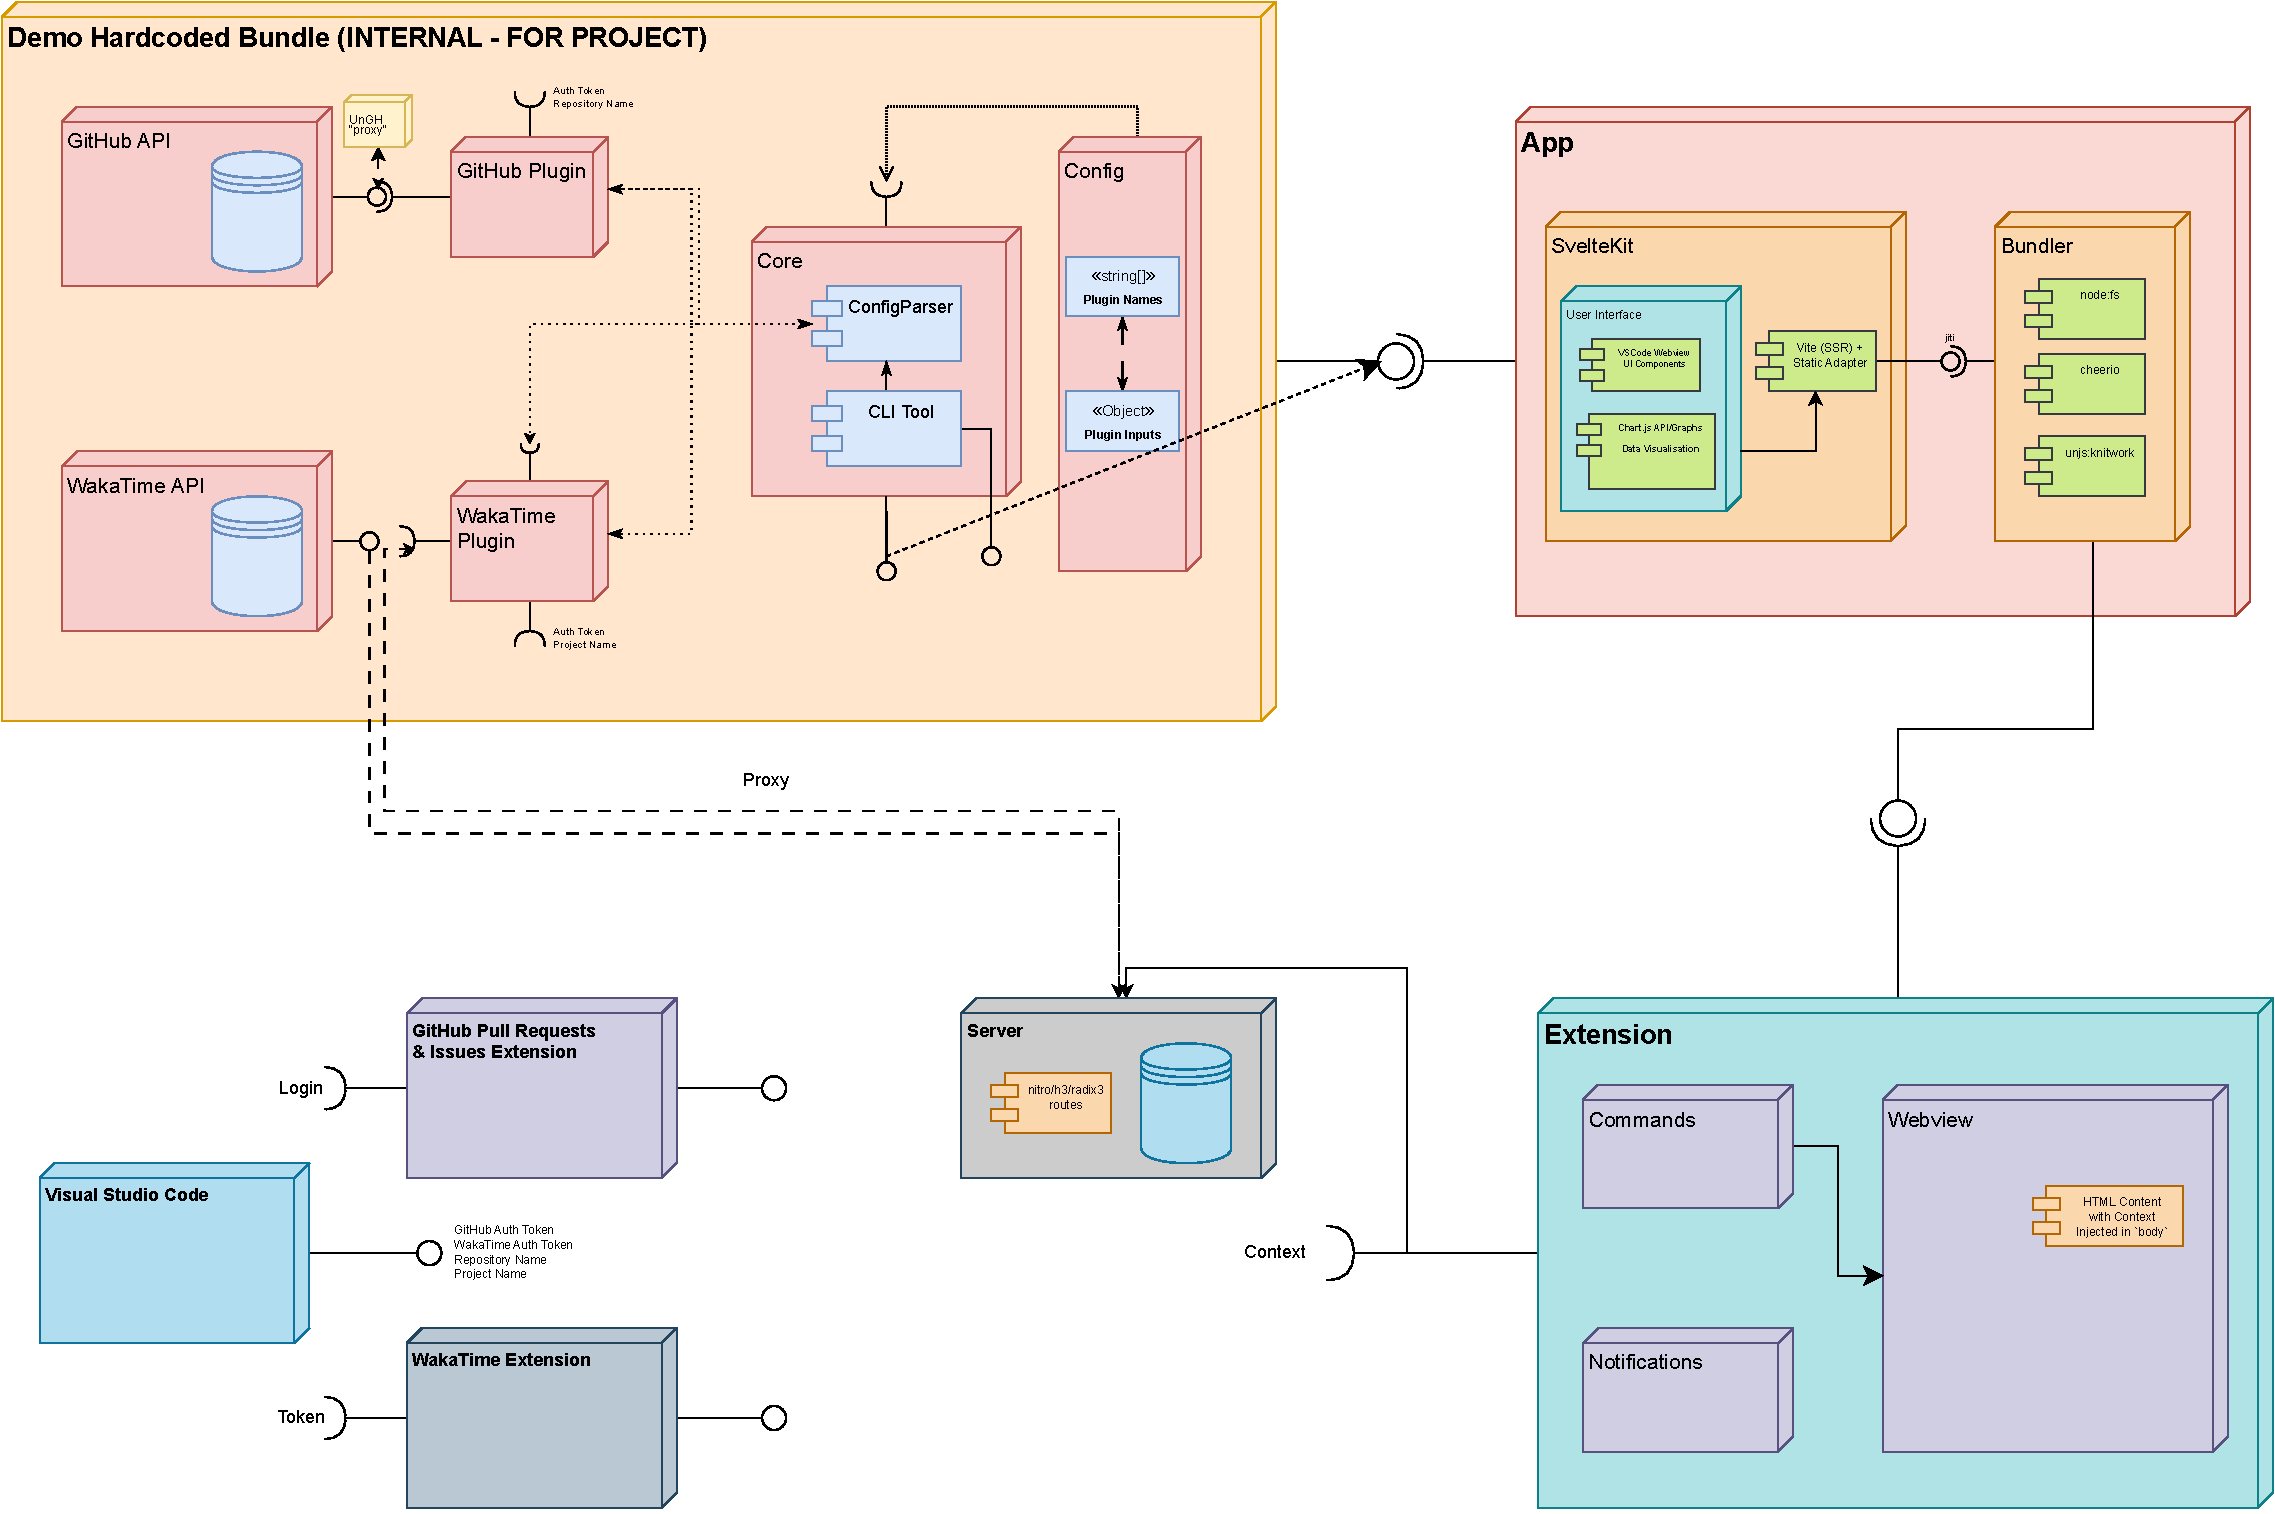
\includegraphics[width=0.5\textwidth]{architecture.pdf}}\end{figure} | 
| --- | --- |

\vspace{-0.5cm}

{\footnotesize
```ts
  async getWebviewContent(webview: Webview, extensionUri: Uri) {
    return appWebview(webview, extensionUri, 'dist')
      .replace('<body ', `<body ${Object.entries({
          // plugin-0 -> github, plugin-1 -> wakatime
          'github-repolink': (await Promise.all(
              this.gitExtension?.repositories.map((r) =>
                r.getConfig('remote.origin.url')
              ) || [])).join(),
        }).map(([k, v]) => `data-${kebabCase(k)}="${v}"`)`);
  }
```
}

\vspace{-0.5cm}

| \begin{figure}\textcolor{black}{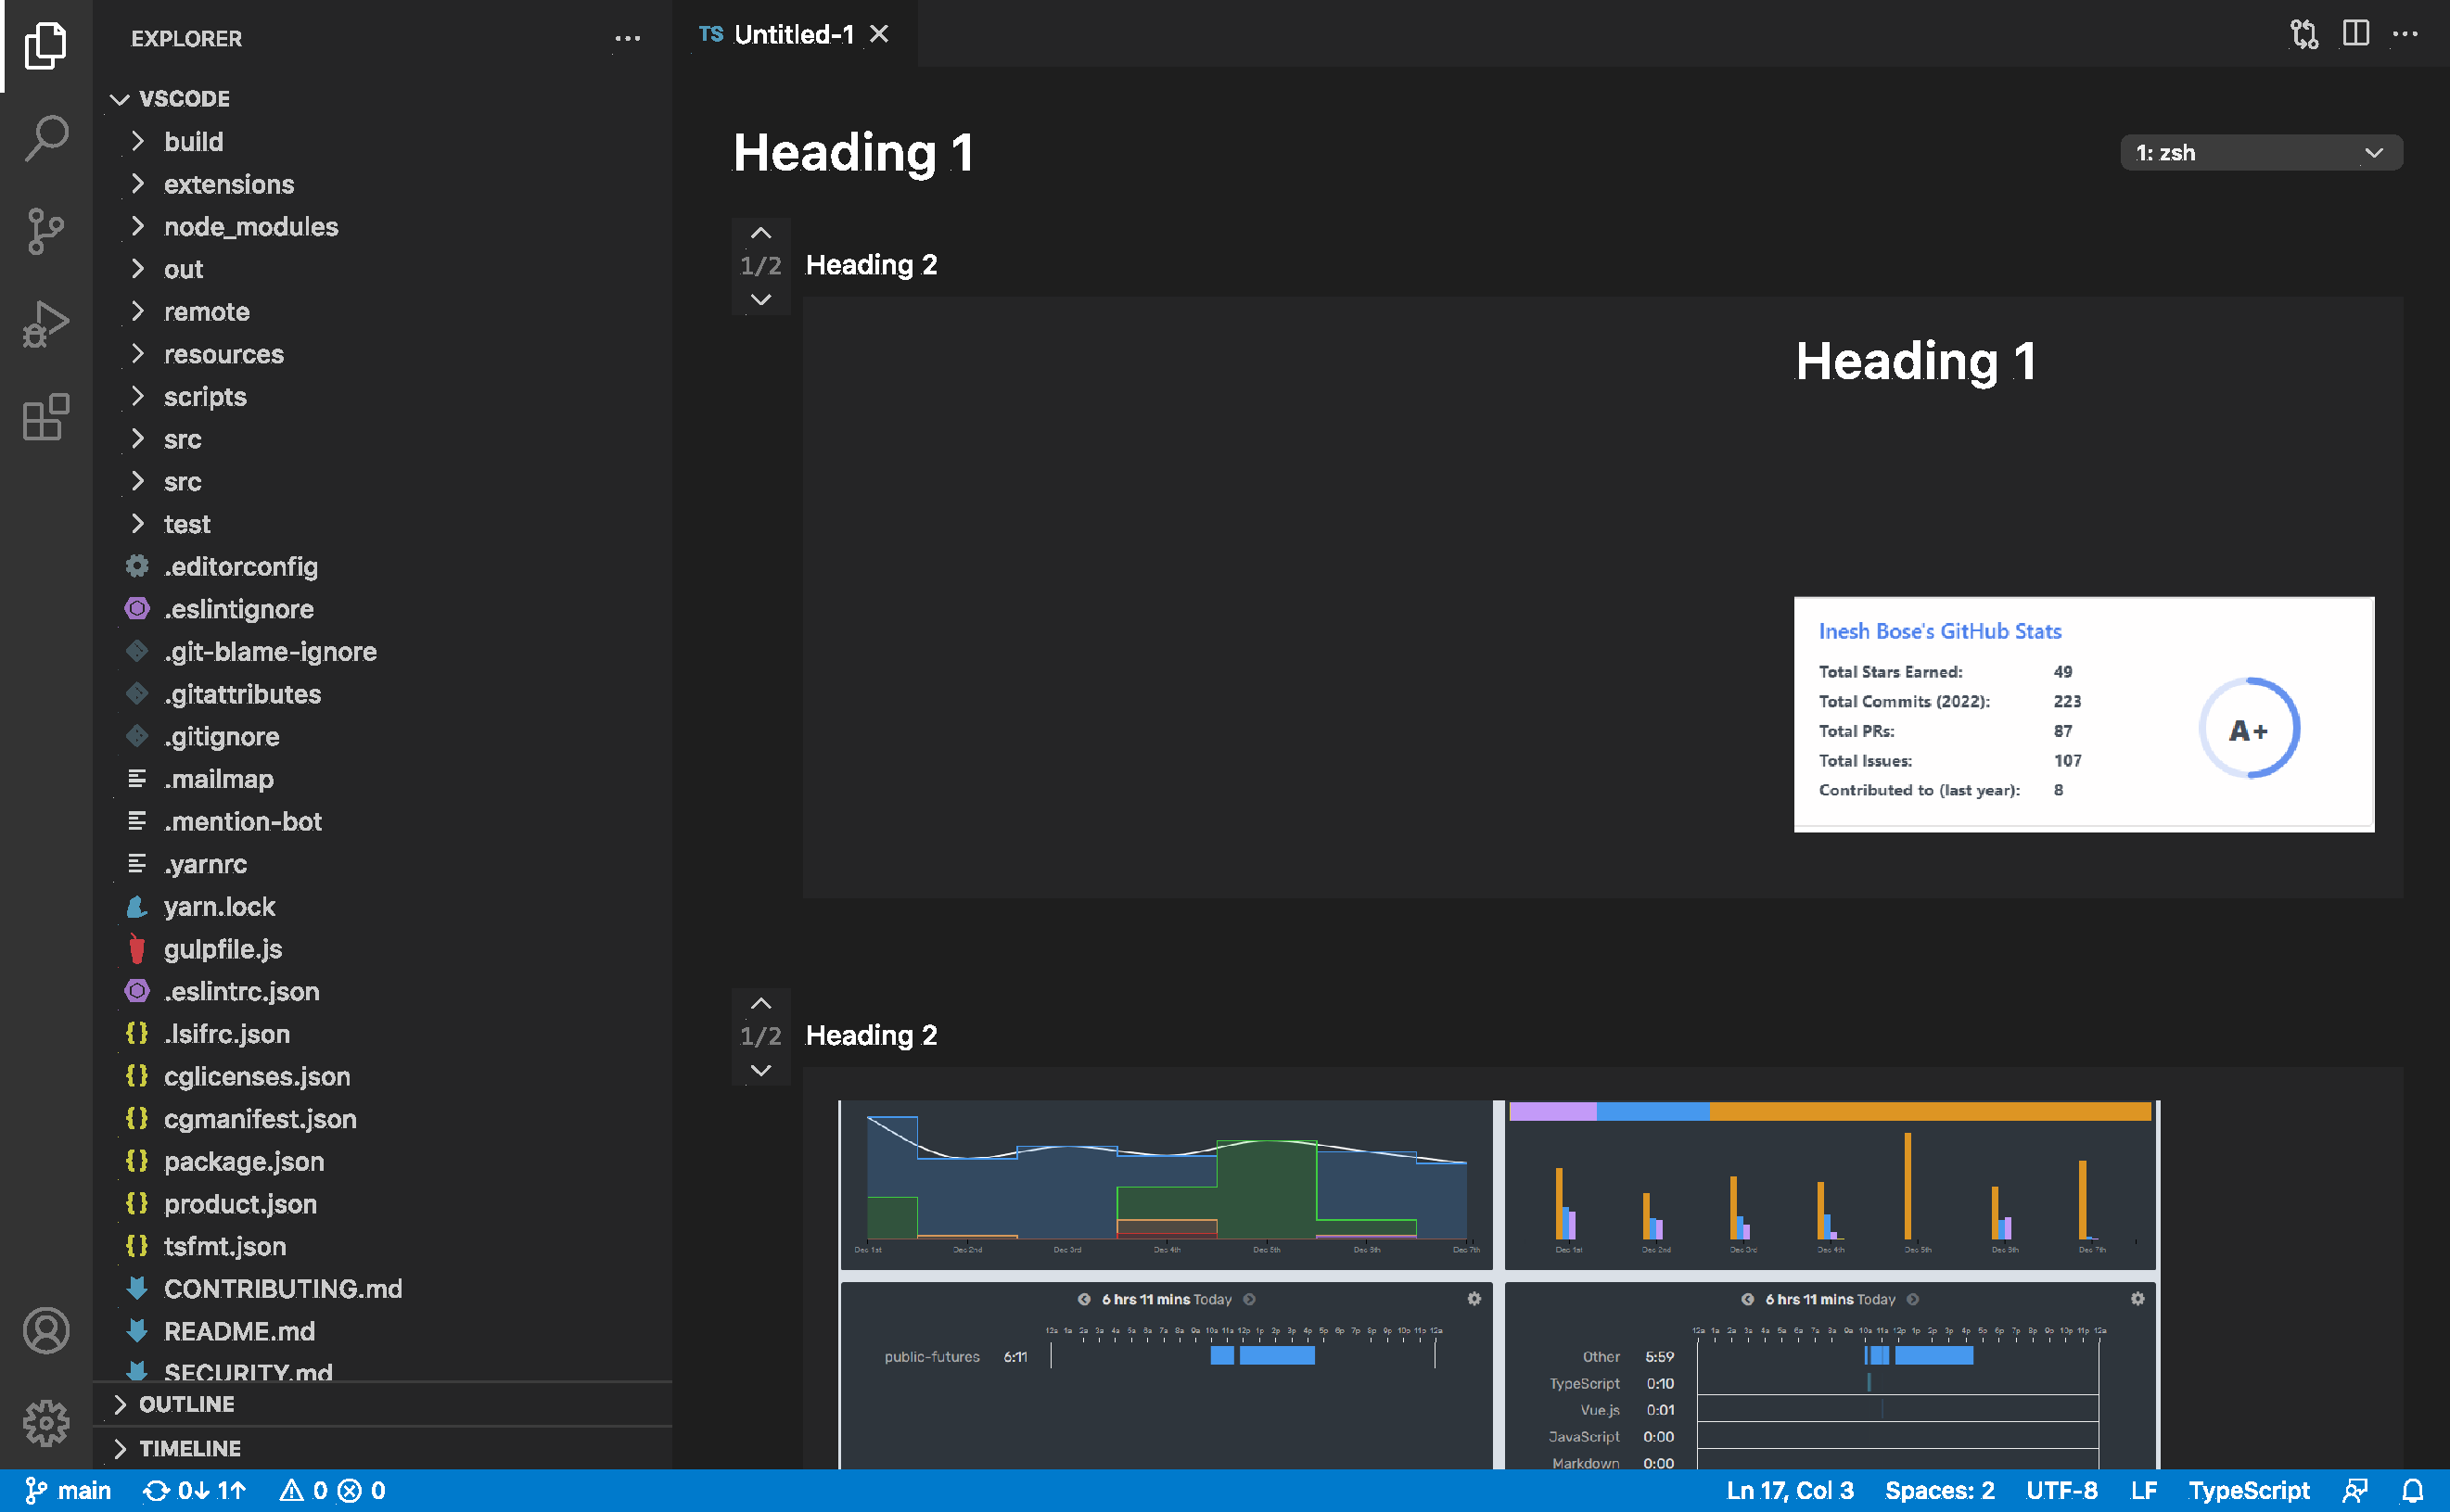
\includegraphics[width=0.4\textwidth]{initialwf.pdf}}\end{figure} | \begin{figure}\textcolor{black}{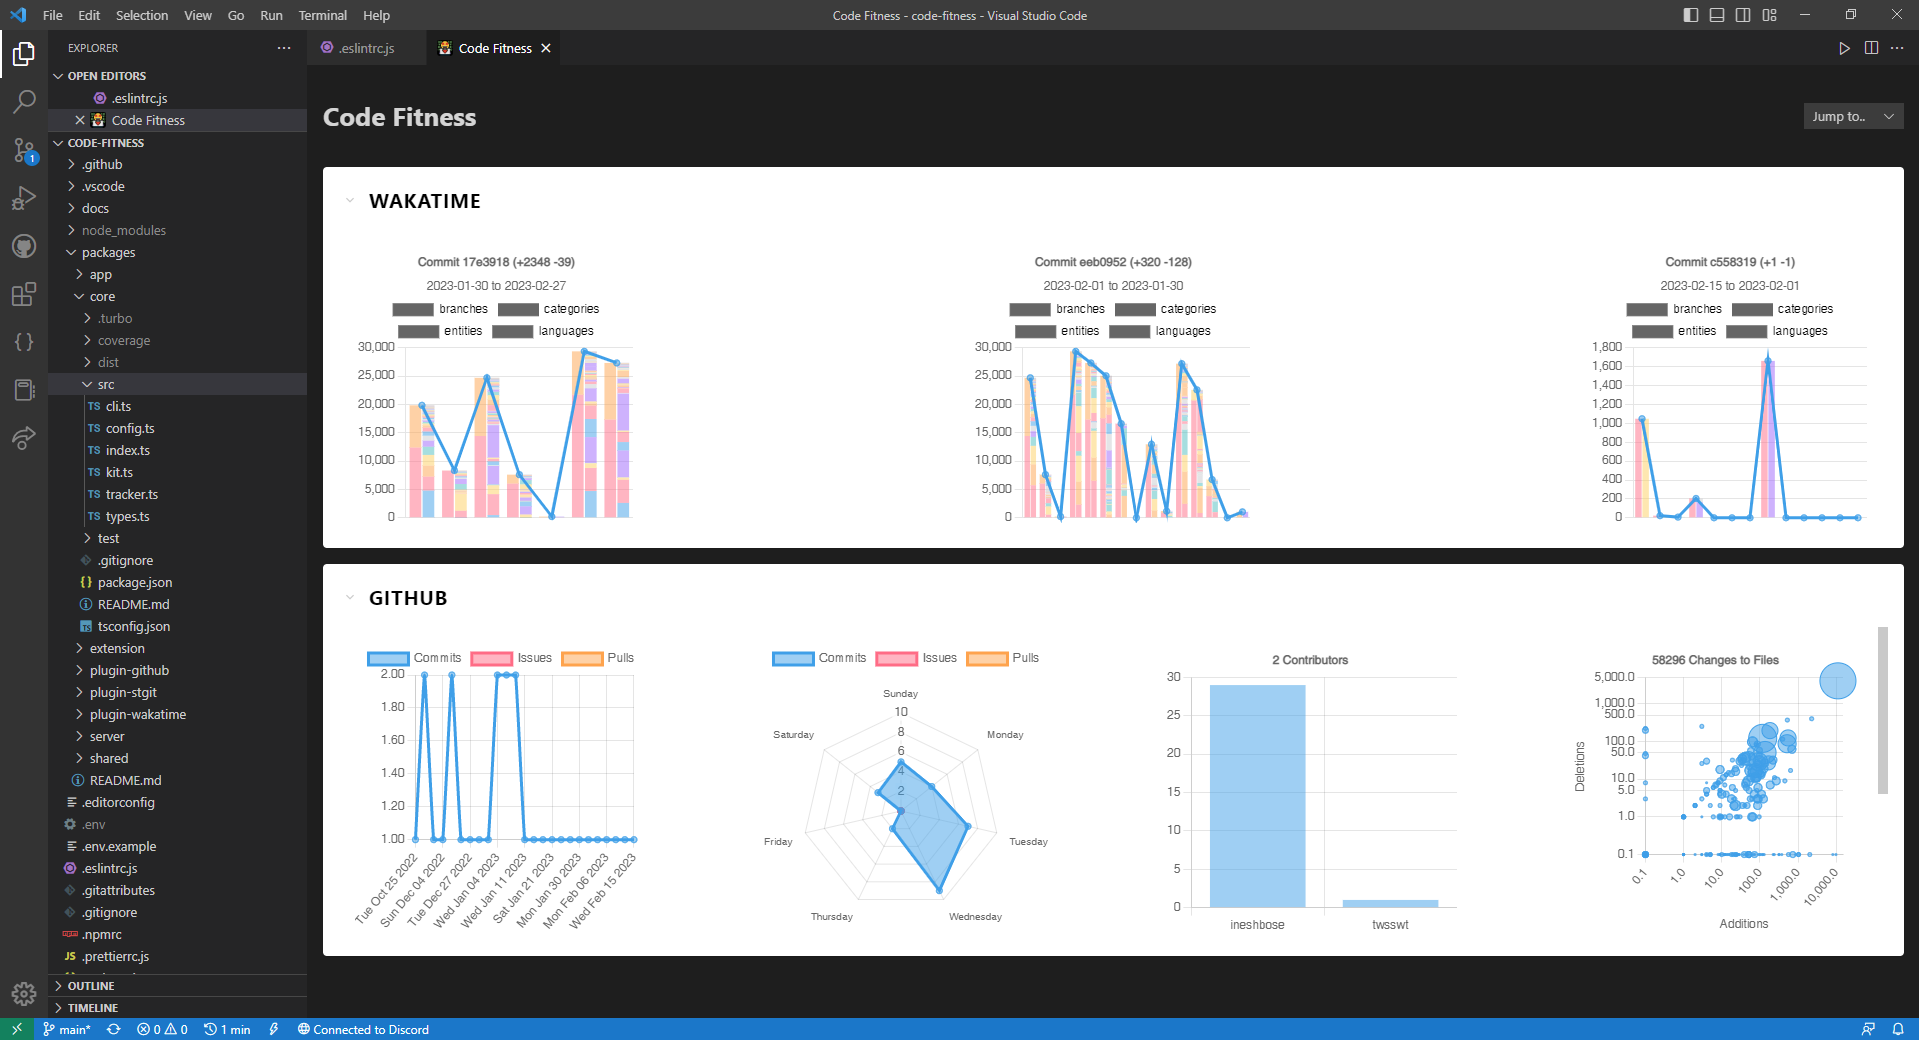
\includegraphics[width=0.45\textwidth]{screenshot_27-02.png}}\end{figure} | 
| --- | --- |

\vspace{-0.5cm}

----

\end{markdown}

\end{column}

%%%% Second Column
\begin{column}{.48\textwidth}

\begin{markdown}

#### Research Objectives %{\scriptsize the goal?}

\footnotesize

- To evaluate task estimations carried by software developers and outline points of frustration along with the potential for improvements.
- To provide developers with visualisations of more suitable \& realistic measures from their development activity that occurs as \textit{continuous} events between the \textit{discrete} commits of their code repository.
- To develop \& provide a dashboard using a \textit{modular} architecture that is \textit{integrated} into different systems and into developers' workflow.

----

% #### Evaluation \& Conclusion {\scriptsize the findings?}

% \footnotesize

% Teams customised the dashboard for personalised metrics - most opting to see how much time was spent browsing docs \& StackOverflow. Over the weeks, future tasks had more accurate and educated estimates.

% \vspace{0.5cm}

% \centering
% \begin{tikzpicture}[scale=0.8]
% \begin{axis}[    xlabel={Week Number},    ylabel={Hours per task (avg)},    xmin=1, xmax=8,    ymin=0, ymax=20,    xtick={1,2,3,4,5,6,7,8},    ytick={0,10,20,30,40},    legend pos=north west,    ymajorgrids=true,    grid style=dashed,    axis line style={white},    tick style={white},    xtick style={white},    ytick style={white},    xlabel style={white},    ylabel style={white},    clip marker paths=true, xticklabel style={color=white}, yticklabel style={color=white}, legend columns=2, width=1\textwidth,    height=0.4\textwidth, legend style={        cells={align=left},        fill=none,        draw=none,        font=\footnotesize,    },    legend image post style={sharp plot,|-|,line width=.5pt}]

% \addplot[    color=red,    mark=none,    smooth,    tension=0.5,    fill=red!50,   fill opacity=0.3,   ]
%     coordinates {
%     (1,15)(2,7)(3,14)(4,12)(5,16)(6,10)(7,14)(8,12)
%     } \closedcycle;

% \addplot[    color=blue!80,    mark=none,    smooth,    tension=0.5,    fill=blue!50,  fill opacity=0.3,  ]
%     coordinates {
%     (1,8)(2,10)(3,6)(4,15)(5,14)(6,11)(7,14)(8,12)
%     } \closedcycle;
%     \legend{\textcolor{white}{Actual},\textcolor{white}{Estimate}}

% \end{axis}
% \end{tikzpicture}

% ----

#### Bibliography

\bibliographystyle{unsrtnat}
\renewcommand*{\bibfont}{\scriptsize}
\bibliography{docs/references/primary,docs/references/secondary,docs/references/tertiary,docs/references/technology,docs/references/repository}

\vspace{0.2cm}

{\footnotesize See the repository on \texttt{\scriptsize \href{https://github.com/ineshbose/code-fitness}{github.com/ineshbose/code-fitness}}}

----

\end{markdown}
\end{column}
\end{columns}
\end{frame}


\end{document}